\documentclass{hw_template}

\usepackage{arydshln}

\title{\bfseries Домашня Робота \#4 з Теорії Коливань}
\author{\bfseries Захаров Дмитро}
\date{16 березня, 2025}

\begin{document}

\pagestyle{fancy}

\maketitle

\section{Задача 3}


\begin{problem}
    Визначте частоти і форми малих коливань у вертикальній площині однорідного
стержня довжини $L=2\ell$, прив’язаного до нитки довжини $\ell$.
\end{problem}

\begin{center}
    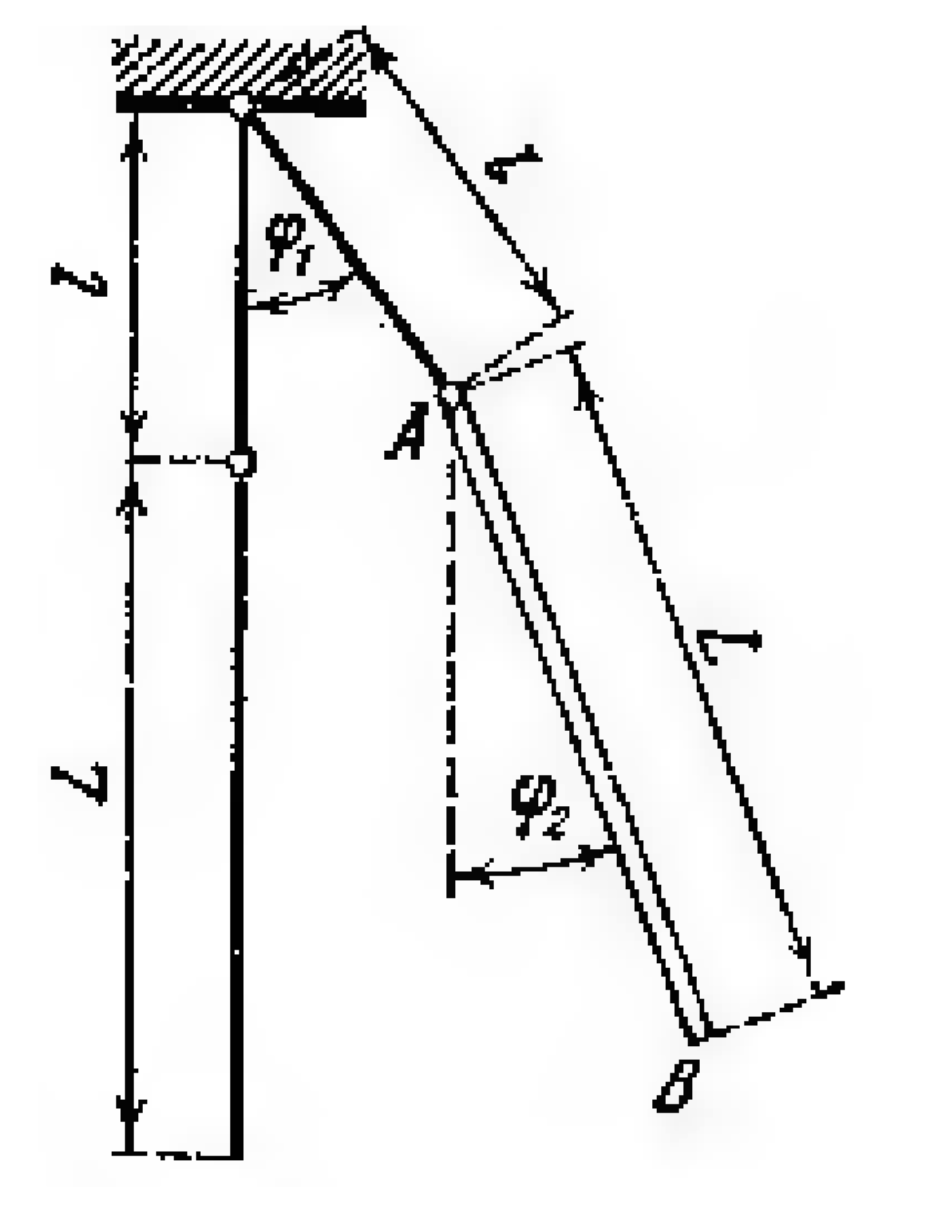
\includegraphics[width=0.3\linewidth]{images/hw_4_problem_3.png}
\end{center}

\textbf{Розв'язання.} Нехай, як і на малюнку, амплітуди кутів відхилення від
вертикалі дорівнюють $\varphi_1$ та $\varphi_2$. Початкова потенціальна енергія
$\Pi_0 = -2mg\ell$. Оскільки масою нитки ми нехтуємо, то потенціальна енергія в 
такому разі:
\begin{equation*}
    \Pi(\varphi_1, \varphi_2) = -mg\ell\cos\varphi_1 - mg\ell\cos\varphi_2 = -mg\ell(\cos\varphi_1 + \cos\varphi_2)
\end{equation*}

Таким чином, зміна потенціальної енергії:
\begin{align*}
    \Delta \Pi(\varphi_1, \varphi_2) &= 2mg\ell - mg\ell(\cos\varphi_1 + \cos\varphi_2) \\
    &= mg\ell((1-\cos\varphi_1) + (1-\cos\varphi_2)) \\
    &\approx \frac{1}{2}mg\ell\varphi_1^2 + \frac{1}{2}mg\ell\varphi_2^2
\end{align*}

Цікавіша ситуація з кінетичною енергією. Вона складаєтсья з обертальної
кінетичної енергії стержня та кінетичної енергії руху центра мас. Кінетична
енергія обертального руху може бути записана як $T_{\text{rot}} =
\frac{1}{2}I\dot{\varphi}_2$, де $I$ - момент інерції стержня, $I =
\frac{1}{12}m(2\ell)^2 = \frac{1}{3}m\ell^2$, тому $T_{\text{rot}} =
\frac{1}{6}m\ell^2\dot{\varphi}_2$.

Розберемося з кінетичною енергією руху центра мас. Виразимо координати 
центра мас стержня:
\begin{align*}
    x_C &= \ell(\sin\varphi_1 + \sin\varphi_2), \\
    y_C &= -\ell(\cos\varphi_1 + \cos\varphi_2)
\end{align*}

Похідні по часу:
\begin{align*}
    \dot{x}_C &= \ell(\dot{\varphi}_1\cos\varphi_1 + \dot{\varphi}_2\cos\varphi_2), \\
    \dot{y}_C &= \ell(\dot{\varphi}_1\sin\varphi_1 + \dot{\varphi}_2\sin\varphi_2)
\end{align*}

Модуль швидкості можна знайти як $v_C=\sqrt{\dot{x}_C^2+\dot{y}_C^2}$, тому
\begin{align*}
    v_C^2 &= \ell^2(\dot{\varphi}_1^2\cos^2\varphi_1 + 2\dot{\varphi}_1\cos\varphi_1\dot{\varphi}_2\cos\varphi_2 + \dot{\varphi}_2^2\cos^2\varphi_2
    \\&+ \dot{\varphi}_1^2\sin^2\varphi_1 + 2\dot{\varphi}_1\sin\varphi_1\dot{\varphi}_2\sin\varphi_2 + \dot{\varphi}_2^2\sin^2\varphi_2) \\
    &= \ell^2(\dot{\varphi}_1^2 + \dot{\varphi}_2^2 + 2\dot{\varphi}_1\dot{\varphi}_2(\cos\varphi_1\cos\varphi_2 + \sin\varphi_1\sin\varphi_2)) \\
    &= \ell^2(\dot{\varphi}_1^2 + \dot{\varphi}_2^2 + 2\dot{\varphi}_1\dot{\varphi}_2\cos(\varphi_1 - \varphi_2))
\end{align*}

Проте, цей вираз, взагалі кажучи, не є квадратичною формою відносно
$(\dot{\varphi}_1,\dot{\varphi_2})$, оскільки нам треба ще скористатися малістю
$\varphi_1$, $\varphi_2$. Для чого скористаємося наближенням $\cos\varphi_i \approx 1-\frac{\varphi_i^2}{2}$,
та $\sin\varphi_i \approx \varphi_i$. Тоді:
\begin{align*}
    \cos\varphi_1\cos\varphi_2 + \sin\varphi_1\sin\varphi_2 &\approx \left(1-\frac{\varphi_1^2}{2}\right)\left(1-\frac{\varphi_2^2}{2}\right) + \varphi_1\varphi_2 \\
    &\approx 1 + \varphi_1\varphi_2 - \frac{\varphi_1^2+\varphi_2^2}{2} = 1 - \frac{(\varphi_1-\varphi_2)^2}{2}
\end{align*}

(тут ми відкинули $\frac{1}{4}\varphi_1^2\varphi_2^2$ у силу малості). Таким
чином, отримуємо:
\begin{equation*}
    v_C^2 \approx \ell^2\left(\dot{\varphi}_1^2 + \dot{\varphi}_2^2 + 2\dot{\varphi}_1\dot{\varphi}_2\left(1 - \frac{(\varphi_1-\varphi_2)^2}{2}\right)\right) = \ell^2((\dot{\varphi}_1+\dot{\varphi}_2)^2 - \dot{\varphi}_1\dot{\varphi}_2(\varphi_1-\varphi_2)^2)
\end{equation*}

Оскільки вираз $\dot{\varphi}_1\dot{\varphi}_2(\varphi_1-\varphi_2)^2$ наближено
має четвертий порядок малості, то остаточно отримуємо $v_C \approx
\ell(\dot{\varphi}_1+\dot{\varphi}_2)$. Таким чином,
\begin{equation*}
    T(\dot{\varphi}_1,\dot{\varphi}_2) = \frac{1}{2}mv_C^2 + \frac{1}{6}m\ell^2\dot{\varphi}_2^2 \approx \frac{1}{2}m\ell^2(\dot{\varphi}_1+\dot{\varphi}_2)^2 + \frac{1}{6}m\ell^2\dot{\varphi}_2^2
\end{equation*}

Тепер, запишемо як потенціальну, так і кінетичну енергію у вигляді квадратичної форми. 
Для потенціальної енергії все доволі просто:
\begin{equation*}
    \Pi(\varphi_1,\varphi_2) = \frac{1}{2}\varphi^{\top}A_{\Pi}\varphi, \quad A_{\Pi} = \begin{pmatrix}
        mg\ell & 0 \\
        0 & mg\ell
    \end{pmatrix}
\end{equation*}

З кінетичною енергією, розкриємо дужки:
\begin{equation*}
    T(\dot{\varphi}_1,\dot{\varphi}_2) = \frac{1}{2}m\ell^2\dot{\varphi}_1^2 + m\ell^2\dot{\varphi}_1\dot{\varphi}_2 + \frac{2}{3}m\ell^2\dot{\varphi}_2^2
\end{equation*}

Таким чином, квадратична форма:
\begin{equation*}
    T(\dot{\varphi}_1,\dot{\varphi}_2) = \frac{1}{2}\dot{\varphi}^{\top}A_T\dot{\varphi}, \quad A_T = \begin{pmatrix}
        m\ell^2 & m\ell^2 \\
        m\ell^2 & \frac{4}{3}m\ell^2
    \end{pmatrix}
\end{equation*}

Для аналізу частот, знайдемо розв'язок рівняння $\det(-\omega^2A_T +
A_{\Pi})=0$:
\begin{equation*}
    -\omega^2A_T + A_{\Pi} = \begin{pmatrix}
        mg\ell - m\ell^2\omega^2 & -m\ell^2\omega^2 \\
        -m\ell^2\omega^2 & mg\ell - \frac{4}{3}m\ell^2\omega^2
    \end{pmatrix} = \begin{pmatrix}
        1 - \frac{\omega^2}{\Omega^2} & -\frac{\omega^2}{\Omega^2} \\
        -\frac{\omega^2}{\Omega^2} & 1 - \frac{4}{3}\frac{\omega^2}{\Omega^2}
    \end{pmatrix}mg\ell,
\end{equation*}

де $\Omega^2 = g/\ell$ --- величина з розмірністю частоти для позбавлення 
від одиниць вимірності. Тоді, визначник:
\begin{equation*}
    \left(1 - \frac{\omega^2}{\Omega^2}\right)\left(1 - \frac{4}{3}\frac{\omega^2}{\Omega^2}\right) - \frac{\omega^4}{\Omega^4} = 0
\end{equation*}

Розкриваємо дужки:
\begin{equation*}
    \frac{1}{3} \frac{\omega^4}{\Omega^4}- \frac{7}{3} \frac{\omega^2}{\Omega^2} + 1 = 0
\end{equation*}

Якщо позначити $\xi := \omega^2/\Omega^2$, то отримуємо рівняння
$\xi^2-7\xi+3=0$, звідки $\xi = \frac{7 \pm \sqrt{37}}{2}$. Оскільки $\sqrt{37}
\approx \sqrt{36}=6$, то наближено $\xi_1 = \frac{13}{2}$ та $\xi_2 =
\frac{1}{2}$. Таким чином, наближено, $\omega_1 \approx \sqrt{\frac{13g}{2\ell}}$ та
$\omega_2 \approx \sqrt{\frac{g}{2\ell}}$ або $\omega_1 \approx 2.56\sqrt{\frac{g}{\ell}}$
та $\omega \approx 0.68\sqrt{\frac{g}{\ell}}$.

Для знаходження $\varphi_2/\varphi_1$ при кожній частоті, достатньо знайти
власні вектори матриці $-\omega_i^2A_T + A_{\Pi}$ для $i=1,2$, а далі знайти
відношення їх компонент. Для $\omega_1$ маємо власний вектор $(-0.763,0.646)$,
тому відношення $\varphi_1/\varphi_2 = -0.763/0.646 \approx -1.18$. Для
$\omega_2$ аналогічно маємо $\varphi_1/\varphi_2 \approx 0.85$.

\end{document}